\documentclass[11pt,a4paper,twoside]{tesis}
% SI NO PENSAS IMPRIMIRLO EN FORMATO LIBRO PODES USAR
%\documentclass[11pt,a4paper]{tesis}

\usepackage{graphicx}
\usepackage{amssymb}
\usepackage{amsmath}
\usepackage{amsthm}
\usepackage[utf8]{inputenc}
\usepackage[spanish]{babel}
\usepackage[left=3cm,right=3cm,bottom=3.5cm,top=3.5cm]{geometry}

\begin{document}

%%%% CARATULA
% Comentar y descomentar según corresponda
\def\titulo{Licenciado }

\def\autor{Juan Manuel Pérez}
\def\tituloTesis{Mimetización entre interlocutores}
\def\runtitulo{Medición de la mimetización entre interlocutores utilizando series de tiempo}
\def\runtitle{Measuring entrainment between speakers using time series}
\def\director{Agustín Gravano}
\def\codirector{Ramiro Gálvez}
\def\lugar{Buenos Aires, 2015}
\newcommand{\HRule}{\rule{\linewidth}{0.2mm}}
%
\thispagestyle{empty}

\begin{center}\leavevmode

\vspace{-2cm}

\begin{tabular}{l}

\includegraphics[width=2.6cm]{logofcen.pdf}
\end{tabular}


{\large \sc Universidad de Buenos Aires

Facultad de Ciencias Exactas y Naturales

Departamento de Computaci\'on}

\vspace{6.0cm}

%\vspace{3.0cm}
%{
%\Large \color{red}
%\begin{tabular}{|p{2cm}cp{2cm}|}
%\hline
%& Pre-Final Version: \today &\\
%\hline
%\end{tabular}
%}
%\vspace{2.5cm}

{\huge\bf \tituloTesis}

\vspace{2cm}

{\large Tesis de \titulo en Ciencias de la Computaci\'on}

\vspace{2cm}

{\Large \autor}

\end{center}

\vfill

{\large

{Director: \director}

\vspace{.2cm}

{Codirector: \codirector}

\vspace{.2cm}

\lugar
}

% \newpage\thispagestyle{empty}


%%%% ABSTRACTS, AGRADECIMIENTOS Y DEDICATORIA
\frontmatter
\pagestyle{empty}
%\begin{center}
%\large \bf \runtitulo
%\end{center}
%\vspace{1cm}
\chapter*{\runtitulo}

\noindent El \emph{entrainment} (mimetización) es un fenómeno inconsciente que se manifiesta a través de la adaptación de posturas, forma de hablar, gestos faciales y otros comportamientos entre dos o más interactores. A su vez, la ocurrencia de esta mimetización está fuertemente emparentada con el sentimiento de empatía y compenetración entre los participantes.

En esta tesis, nos proponemos explorar una técnica algorítmica para detectar el entrainment entre variables prosódicas de dos personas. Esta técnica nos permitirá determinar si existe o no convergencia para ciertos parámetros, y ver como está esto correlacionado con variables sociales tales como la empatía, la compenetración con la tarea, y otras.

\bigskip

\noindent\textbf{Palabras claves:} Guerra, Rebelión, Wookie, Jedi, Fuerza, Imperio (no menos de 5).

%\begin{center}
%\large \bf \runtitle
%\end{center}
%\vspace{1cm}
\chapter*{\runtitle}

\noindent In a galaxy far, far away, a psychopathic emperor and his most trusted servant -- a former Jedi Knight known as Darth Vader -- are ruling a universe with fear. They have built a horrifying weapon known as the Death Star, a giant battle station capable of annihilating a world in less than a second. When the Death Star's master plans are captured by the fledgling Rebel Alliance, Vader starts a pursuit of the ship carrying them. A young dissident Senator, Leia Organa, is aboard the ship \& puts the plans into a maintenance robot named R2-D2. Although she is captured, the Death Star plans cannot be found, as R2 \& his companion, a tall robot named C-3PO, have escaped to the desert world of Tatooine below. Through a series of mishaps, the robots end up in the hands of a farm boy named Luke Skywalker, who lives with his Uncle Owen \& Aunt Beru. Owen \& Beru are viciously murdered by the Empire's stormtroopers who are trying to recover the plans, and Luke \& the robots meet with former Jedi Knight Obi-Wan Kenobi to try to return the plans to Leia Organa's home, Alderaan. After contracting a pilot named Han Solo \& his Wookiee companion Chewbacca, they escape an Imperial blockade. But when they reach Alderaan's coordinates, they find it destroyed - by the Death Star. They soon find themselves caught in a tractor beam \& pulled into the Death Star. Although they rescue Leia Organa from the Death Star after a series of narrow escapes, Kenobi becomes one with the Force after being killed by his former pupil - Darth Vader. They reach the Alliance's base on Yavin's fourth moon, but the Imperials are in hot pursuit with the Death Star, and plan to annihilate the Rebel base. The Rebels must quickly find a way to eliminate the Death Star before it destroys them as it did Alderaan (aprox. 200 palabras).

\bigskip

\noindent\textbf{Keywords:} War, Rebellion, Wookie, Jedi, The Force, Empire (no menos de 5).

\tableofcontents

\mainmatter
\pagestyle{headings}

%%%% ACA VA EL CONTENIDO DE LA TESIS

\chapter{Introducción}

\section{Introducción}

Los sistemas de diálogo humano-computadora son cada vez más frecuentes, y sus aplicaciones comprenden una amplia gama de rubros: desde aplicaciones móviles, motores de búsqueda, juegos, o tecnologías de asistencia para ancianos y discapacitados.

Si bien es cierto que estos sistemas logran captar la dimensión lingüística de la comunicación humana, tienen un déficit importante a la hora de procesar y transmitir el aspecto superestructural de la comunicación, que radica en el intercambio de afecto, emociones, actitudes y otras intenciones de los participantes. La habilidad de los participantes de poder expresar, comprender, y reaccionar de acuerdo a estas señales sociales es necesaria para el entendimiento mutuo y una comunicación exitosa.

Un aspecto particular de la comunicación es el fenómeno de \emph{entrainment}(arrastre, mimetización, efecto camaleón), que comprende la adaptación inconsciente de las variables acústicas/prosódicas(a/p) (por ejemplo, el tono de la voz, la velocidad del habla, etc) de manera dinámica en el transcurso de una o varias interacciones. Este fenómeno ha sido introducido por \emph{Brennan et al}\cite{BRE1996} en 1996, y se ha observado que la convergencia de los participantes en estas variables ocurre en conjunto con una interacción más fluída y un mayor sentimiento de simpatía por sus interlocutores \cite{CHAR1999}.

Poder medir esta mimetización de los interlocutores no es una tarea fácil, sin embargo. En primer lugar, un diálogo no es una sucesión de turnos, sino que es una serie de tiempo dinámica, llena de interrupciones. Más aún, la mimetización no tiene un carácter instantáneo, sino que se sucede a lo largo de la interacción entre los participantes. Estos factores dificultan ostensiblemente poder modelar este fenómeno.


\section{Series de Tiempo}
\label{sec:time_series}
\nota{Mandar ésto a un apéndice!}

\theoremstyle{definition}
\newtheorem{definicion}{Definición}

\subsection*{Definición Informal}
En términos informales, una serie de tiempo es un conjunto de datos recolectados secuencialmente en el tiempo. Este tipo de datos se dan en varios campos de estudio, como por ejemplo Economía, Ciencias de la Atmósfera, y otros.

Ejemplos de series de tiempo:

\begin{itemize}
    \item Volumen de lluvias en sucesivos días de un año
    \item Precio de acciones en diferentes meses
    \item Cantidad de habitantes de una ciudad año a año
\end{itemize}

\begin{figure}
\centering
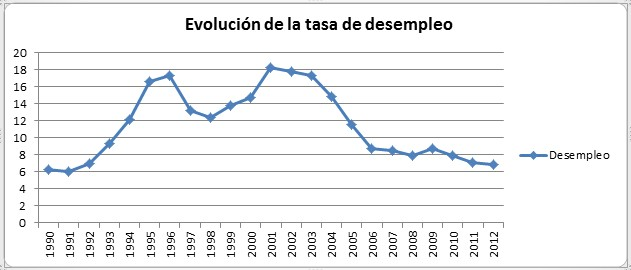
\includegraphics[width=15cm]{images/desocupacion.jpg}
\caption{Gráfico de serie de tiempo de la evolución del desempleo en Argentina \label{desocupacion}}
\end{figure}


\subsection*{¿Para qué queremos series de tiempo?}

Hay varios motivos por los cuales uno querría efectuar un análisis de una serie de tiempo.

\emph{1) Descripción} Usualmente, lo primero que se hace al obtener la serie de tiempo es graficarla y obtener las características más notorias de ésta. Por ejemplo, en \ref{desocupacion} puede notarse que hay una tendencia decreciente del $2003$ hasta el $2012$. En otras (como en el volumen de lluvias) podrá observarse cierta estacionalidad en la serie.

Si bien ésto no requiere técnicas avanzadas de análisis, es el primer paso fundamental para comprender una serie de tiempo.


\emph{2) Explicación} Cuando analizamos dos o más series de tiempo, podemos querer ver cómo se comportan en conjunto. Una variación en una serie de tiempo puede producir un cambio en otra. Por ejemplo, podemos intentar buscar como varían en conjunto la temperatura diaria con la cantidad de mL de lluvia caídos.

\emph{3) Predicción} Dada una serie de tiempo, podemos querer intentar predecir un valor futuro.

\emph{4) Control} Dado un proceso del que se mide cierto parámetro de calidad, podemos querer ajustar variables de entrada para mantenerla en ciertos valores.

En nuestro caso, nos es de interés 1 y 2.


\subsection{Procesos estocásticos}

\begin{definicion}
Una proceso estocástico es una colección de variables aleatorias $\{X_t \}_{t \in T}$ donde $T$ es un conjunto de puntos de tiempo. En nuestro caso, nos interesa $T = \mathbb{N}$, de manera que el proceso será de la forma $X_1, X_2, \ldots $
\end{definicion}

Podemos entender un proceso estocástico como un conjunto de variables ordenadas por el tiempo. Llamamos serie de tiempo a una observación de este proceso estocástico. Usualmente sólo tendremos esta instancia, a diferencia de otros problemas estadísticos donde tendremos muchas observaciones.


\subsection{Estacionariedad}

Un concepto importante en series de tiempo es el de estacionariedad. En lenguaje coloquial, una serie de tiempo estacionaria es aquella en la que no observamos cambios sistemáticos de ésta en el tiempo: si tomamos una parte de la serie, y observamos otro parte distinta de la serie, las propiedades de ésta se mantienen.

Ejemplos de series de tiempo estacionarias son las de ruido blanco, y ejemplos de no estacionarias aquellas que tienen una tendencia. (mejorar esto...)

\begin{definicion}
Un proceso estocástico $X_i, i \in \mathbb{N}$ se dice fuertemente estacionario si, para todo conjunto de índices $t_1, \ldots , t_n$ y para un desplazamiento $\tau \in \mathbb{N}$ tenemos que

\begin{displaymath}
    F_{X_{t_1}, X_{t_2}, \ldots , X_{t_n} } = F_{X_{t_1} + \tau, X_{t_2} + \tau, \ldots , X_{t_n} + \tau}
\end{displaymath}

Es decir, que la función de probabilidad se preserva por traslados.
\end{definicion}

Se derivan como propiedades que, para todo $X_t$ y cualquier desplazamiento $\tau$

\begin{align}
    E[X_t] &= E[X_{t + \tau}] \label{eq:1} \\
    Var[X_t] &= Var[X_{t + \tau}] \label{eq:2} \\
    Cov(X_s, X_t) &= Cov(X_{s+\tau}, X_{t + \tau}) \label{eq:3}
\end{align}

Las ecuaciones \ref{eq:1} y \ref{eq:2} nos dicen que tanto la media como la varianza son constantes (no dependen de $t$), y que la covarianza sólo depende de la diferencia $| s - t |$.


\begin{definicion}
    Un proceso se dice débilmente estacionario si cumple \ref{eq:1}, \ref{eq:2}, \ref{eq:3}
\end{definicion}

A partir de aquí, cuando hablemos de series estacionarias estaremos hablando de series débilmente estacionarias



\section{Columbia Game Corpus}

\newcommand{\objectgame} {\emph{Juego de objetos}}


Empleamos el Columbia Game Corpus  \cite{GRAV2009} consiste en doce conversaciones diádicas (i.e., con dos participantes) entre trece personas angloparlantes distintas. Todos los participantes reportaron hablar Inglés Americano Estándar, y no tener problemas de audición. La edad de los participantes se encuentra en el rango de los 20 a 50 años.

Las grabaciones se hicieron en 44 kHz, 16 bits con un canal separado para cada hablante; luego fueron guardadas en 16 kHz para el presente estudio. Cada sesión duró aproximadamente 45 minutos, totalizando 9 horas de
diálogos, 70.259 palabras (2.037 únicas) para todo el cuerpo de datos.

En cada sesión, se sentó a dos participantes (quienes no se conocían previamente) en una cabina profesional de grabación, cara a cara a ambos lados de una mesa, y con una cortina opaca colgando entre ellos para evitar la comunicación visual. Los participantes contaron con sendas computadoras portátiles conectadas entre sí, en las cuales jugaron una serie de juegos simples que requerían de comunicación verbal. El primero de ellos, un juego de cartas que no consideramos en el presente estudio por tratarse esencialmente de monólogos o diálogos con poca interacción. Luego de esto, pasaron al juego que analizamos, denominado `juego de objetos'.

\subsection{Juego de Objetos}

En el juego de objetos, la pantalla de cada jugador mostró un tablero con varios objetos, entre 5 y 7, como se ve en la figura \ref{objects_game}.
Para uno de los jugadores (el Descriptor) el objeto \emph{Objetivo} aparecía en una posición aleatoria entre otros objetos. Para el otro jugador, a quien llamaremos el Seguidor, el objetivo aparecía en la parte baja de la pantalla. Entonces, al Descriptor se le encargaba describir la posición del Objetivo de manera que el Seguidor pudiera mover su representación del objeto a la misma posición en su pantalla. Luego de una negociación entre ambos jugadores para decidir la mejor posición del objeto, se les asignó a los jugadores una puntuación entre 1 y 100 puntos de acuerdo a qué tan acertado fue el posicionamiento del objetivo por parte del Seguidor.

\begin{figure}
\centering
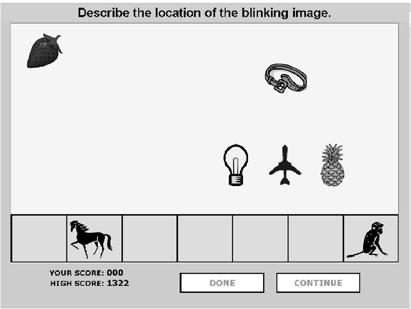
\includegraphics[scale=0.5]{images/columbia_games.jpg}
\caption{Juego de objetos del Columbia Games}
\label{objects_game}
\end{figure}


Cada sesión consistió de 14 tareas como ésta, cambiando los objetos y sus ubicaciones. En las primeras cuatro tareas, uno de los sujetos tomó el papel del Descriptor; en los siguientes cuatro invirtieron roles, y en las finales seis fueron alternando los roles de Descriptor y Seguidor.

\subsection{Anotaciones sobre comportamiento social}

Varios aspectos del comportamiento de los jugadores durante los juegos de objetos fueron anotados mediante la herramienta de crowdsourcing \emph{Amazon Mechanical Turk}. Cada anotador escuchó el audio correspondiente a una tarea del juego y tuvo que responder a varias preguntas sobre cada uno de los sujetos, entre las que se encuentran:

\begin{itemize}
  \item ¿el sujeto parece comprometido con el juego?
  \item ¿el sujeto dirige la conversación?
  \item ¿el sujeto contribuye para el éxito del equipo?
  \item ¿el sujeto alienta a su compañero?
  \item ¿el sujeto se expresa correctamente?
  \item ¿al sujeto no le agrada su compañero?
  \item ¿el sujeto le hace difícil hablar a su compañero?
  \item ¿el sujeto intenta acaparar la conversación?
\end{itemize}

\noindent Cada uno de estos audios fue puntuado por cinco anotadores, que respondieron por sí o por no para cada una de las preguntas. El puntaje que recibe cada una de las preguntas (a las cuales llamaremos a partir de ahora \emph{variables sociales}) consiste en la cantidad de respuestas afirmativas que recibió, teniendo un rango de 0 a 5. Por ejemplo, una tarea dada podría tener puntaje 3 para la variable social `el sujeto A se expresa correctamente' o puntaje 5 para la variable `el sujeto B dirige la conversación'.

\subsection{Extracción de variables acústico/prosódicas}

La herramienta \emph{Praat} fue utilizada para extraer automáticamente las variables \ap del corpus. Las variables que medimos fueron el tono, la intensidad, la proporción de vocalizaciones, jitter, shimmer, cantidad de sílabas, cantidad de fonemas, y la proporción de ruido sobre armónicos. Estos atributos fueron medidos en cada uno de los segmentos de habla del corpus.

Repasemos algunos conceptos que necesitamos para definir las variables acústicas.

\begin{itemize}
  \item \emph{f0} refiere a la frecuencia fundamental de una onda, que es el recíproco del período de ésta. El \emph{tono} o \emph{pitch} es la percepción que tenemos de la frecuencia fundamental, que nos marca cuán agudos o graves son los sonidos.
  \item \emph{Intensity} refiere al volumen o intensidad de la onda. Ésta mide la amplitud de la onda, y es la percepción de cuán fuerte es el sonido.
  \item \emph{jitter y shimmer} se refieren, en un intervalo de tiempo, a los desplazamientos de la onda de la verdadera periodicidad y de la amplitud, respectivamente. Están asociadas con la percepción de la calidad de la voz.
  \item Un \emph{fonema} es la articulación simple de sonidos del habla, tanto de vocales como de consonantes. Ejemplos de fonemas son los sonidos de las letras u, a, s, k en español.
  \item El \emph{noise-to-harmonics ratio} (abreviado NHR) puede considerarse como una medida de calidad de la voz, que cuantifica la proporción de ruido que hay en ésta.
\end{itemize}


En la siguiente tabla resumimos estas features. Recordemos nuevamente que estas features son medidas en un intervalo de tiempo.

\begin{figure}[h!]
\centering
\resizebox{\textwidth}{!}{
\begin{tabular} {|c|c|}
  \hline
  Variable a/p & Descripción \\
  \hline
  \hline
  \FOMEAN & Valor medio de la frecuencia fundamental \\\hline
  \FOMAX  & Valor máximo de la frecuencia fundamental \\\hline
  \ENGMEAN & Valor medio de la intensidad \\\hline
  \ENGMAX & Valor máximo de la intensidad \\\hline
  \NOISETOHARMONICS & Noise-to-harmonics descripto anteriormente \\\hline
  \LOCALSHIMMER & Shimmer medido \\\hline
  \SYLAVG & Cantidad de sílabas por segundo \\\hline
  \PHONAVG & Cantidad de fonemas por segundo \\\hline
\end{tabular}
}
\end{figure}


\section{Método}

\begin{itemize}
\item Selección de Ventanas
\item Time plots, y autocorrelaciones
\end{itemize}

%%%% BIBLIOGRAFIA
\backmatter
\begin{thebibliography}{9}
\bibitem{BRE1996}
    Brennan:
    \emph{Lexical entrainment in spontaneous dialog},
    1996
\bibitem{CHAR1999}
    Chartrand, Bargh:
    \emph{The chameleon effect: The perception-behavior link and social interaction},
    1999
\bibitem{DEL2013}
    De Looze, Scherer, Vaughan, Campbell:
    \emph{Investigating automatic measurements of prosodic accommodation and its dynamics in social interaction},
    2013
\bibitem{KOU2008}
    Kousidis et al:
    \emph{Towards measuring continuous acoustic feature convergence in unconstrained spoken dialogues},
    2008
\bibitem{KOU2009}
    Kousidis, Dorran, McDonnell \& Coyle:
    \emph{Time Series Analysis of Acoustic Feature Convergence in Human Dialogues},
    2009
\bibitem{LEV2012}
    Levitan, Gravano, Willson, Benus, Hirschberg \& Nenkova,
    \emph{Acoustic-Prosodic entrainment and social behavior},
    2012
\bibitem{CHATFIELD}
    Chatfield C.,
    \emph{The analysis of time series: an introduction, Third Edition}
    1984
\end{thebibliography}
\end{document}
